%!TEX root = thesis.tex
\newpage


% \begin{figure}[H]
%   %\centering
%     \subfloat{%
%       \setlength{\unitlength}{0.8cm}
%       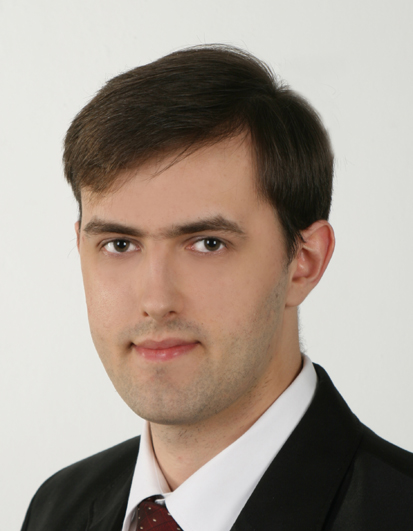
\includegraphics{my-photo.jpg}
%     }
%     \subfloat{
%     	%\begin{flushright}
%     		Kierunek: Informatyka
% 			\vspace{5mm} \\
% 	  		Specjalność: Inżynieria Systemów Informatycznych
% 			\vspace{5mm} \\
% 			Data rozpoczęcia studiów:	2013.10.01
%     	%\end{flushright}      
%     }      
% \end{figure}

\begin{minipage}[t]{0.3\textwidth}
% Pierwsza kolumna
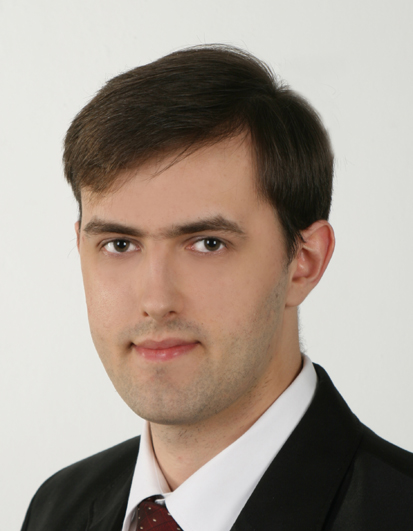
\includegraphics{my-photo.jpg}
\end{minipage}
\begin{minipage}[t]{0.7\textwidth}
\vspace{-45mm}
\emph{Kierunek:} \hspace{10mm} Informatyka
\vspace{5mm} \\
\emph{Specjalność:} \hspace{5mm} Inżynieria Systemów Informatycznych
\vspace{5mm} \\
\emph{Data rozpoczęcia studiów:} \hspace{5mm} 2013.10.01
\end{minipage}

\vspace{10mm} 

\begin{center}
\textbf{Życiorys}
\end{center}

Urodziłem się 7 stycznia 1990 roku w Warszawie. 
Ukończyłem I Liceum Ogólnokształcące im. Wacława Nałkowskiego w Wołominie.
W październiku 2009 roku rozpocząłem studia na Wydziale Elektroniki i Technik Informacyjnch Politechniki Warszawskiej na kierunku Informatyka. W czerwcu 2013 roku uzyskałem tytuł inżyniera. W marcu 2015 roku rozpocząłem roczne praktyki \mbox{w CERN}. 

% Urodziłem się 9 stycznia 1990 roku w Łodzi. W 1997 roku rozpocząłem edukację w Szkole Podstawowej nr 7 w Łodzi. W latach 2003-2006 kontynu- owałem naukę w Gimnazjum nr 42 im. Władysława Stanisława Reymonta w Łodzi. Od 2006 roku uczyłem się w Liceum Ogólnokształcącym nr 31 im. Ludwika Zamenhofa w Łodzi. W 2009 roku zdałem egzaminy maturalne i ukończyłem szkołę licealną z wyróżnieniem. W latach 2009-2013 studiowa- łem dziennie informatykę na Wydziale Elektroniki i Technik Informacyjnych Politechniki Warszawskiej. Ukończyłem studia z wynikiem celującym i ode- brałem tytuł zawodowy inżyniera. Obecnie kończę pracę dyplomową magi- sterską pod kierownictwem Instytutu Informatyki. We wrześniu 2012 roku rozpocząłem pracę zawodową jako programista aplikacji do zarządzania pro- cesami biznesowymi oraz aplikacji mobilnych w firmie Xentivo, gdzie pracuję do dziś. Moją pasją jest tworzenie aplikacji mobilnych oraz internetowych, które uruchamiane są w środowisku iOS.
	 
\begin{flushright}

\dots\dots\dots\dots\dots\dots\dots\dots\dots\dots\dots \\
    \fontsize{9pt}{9pt}\selectfont
      podpis studenta\hspace{18mm}\null
\end{flushright}

\begin{flushleft}
\begin{center}
\vspace{15mm}
\textbf{Egzamin dyplomowy}
\vspace{5mm} \\
\end{center}

Złożył egzamin dyplomowy w dn. \manydots	 
\vspace{5mm} \\
z wynikiem \manydots 	
\vspace{5mm} \\
Ogólny wynik studiów: \manydots	 
\vspace{5mm} \\
Dodatkowe wnioski i uwagi Komisji: \manydots	 
\manydots \\ 
\vspace{5mm}
\manydots
\end{flushleft}
	
\pagenumbering{gobble}
